%==================== PARTIE 2 ====================
\section{Partie 2 : Débruitage d'une harmonique}

On considère $d(n)=\sin(nw_0+\phi)$, $n=1,\dots,N$, avec $N=10^4$, $w_0=0.05\pi$ et $\phi=\pi/4$. Le signal bruité est $x(n)=d(n)+v(n)$, où $v(n)$ est un bruit blanc gaussien $\mathcal{N}(0,\sigma_v^2)$ généré avec \texttt{randn}.

\textbf{Notations.} Le filtre de Wiener d'ordre $P$ estime $d(n)$ à partir du régresseur $\mathbf{x}(n)=[x(n),\,x(n-1),\,\dots,\,x(n-P+1)]^T$ :
\[
\hat d(n)=\mathbf{w}_{opt}^T\mathbf{x}(n),\qquad
\mathbf{w}_{opt}=\mathbf{R}_x^{-1}\mathbf{r}_{dx},\qquad
\mathrm{EQM}_{\min}=r_d(0)-\mathbf{w}_{opt}^T\mathbf{r}_{dx},
\]
où $\mathbf{R}_x$ est la matrice de Toeplitz construite sur $r_x(0),\dots,r_x(P-1)$ et $\mathbf{r}_{dx}=[r_{dx}(0),\dots,r_{dx}(P-1)]^T$. Comme $d$ et $v$ sont indépendants et $v$ centré : $r_x(k)=r_d(k)+\sigma_v^2\,\delta(k)$ et $r_{dx}(k)=r_d(k)$.

\subsection{Question (a) : affichage des signaux}

\begin{enonce}
\textbf{Énoncé :} Afficher une fenêtre de $d(n)$, $x(n)$ et $\hat d(n)$ pour $P=10$ et $\sigma_v^2=0.1$.
\end{enonce}

\textbf{Démarche.}
\begin{enumerate}
  \item Génération de $d(n)$, de $v(n)=\sqrt{\sigma_v^2}\,\texttt{randn}$ et de $x(n)=d(n)+v(n)$.
  \item Estimation de $r_x(k)$ et $r_{dx}(k)=r_d(k)$ par moyennes temporelles (\texttt{xcorr}, retards $0$ à $P-1$).
  \item Construction de $\mathbf{R}_x$ (\texttt{toeplitz}) et résolution de $\mathbf{R}_x\mathbf{w}_{opt}=\mathbf{r}_{dx}$.
  \item Filtrage : $\hat d(n)=\mathbf{w}_{opt}^T\mathbf{x}(n)$ (\texttt{filter}).
\end{enumerate}

\textbf{Code.}
\begin{lstlisting}
clear; clc; close all;

% Parametres
N     = 1e4;          % nombre d'echantillons
n     = (1:N)';
w0    = 0.05*pi;
phi   = pi/4;         % phase fixee
P     = 10;           % ordre du filtre
sigv2 = 0.1;          % variance du bruit

% Signal, bruit, signal bruite
d = sin(n*w0 + phi);
v = sqrt(sigv2)*randn(N,1);
x = d + v;

% Correlations (retards 0 a P-1) : r_dx(k) = r_d(k)
rx = xcorr(x, P-1, 'biased');  rx = rx(P:end);
rd = xcorr(d, P-1, 'biased');  rd = rd(P:end);
Rx = toeplitz(rx);

% Filtre de Wiener et signal debruite
wopt = Rx \ rd;
dhat = filter(wopt, 1, x);

% Affichage d'une fenetre
idx = 101:200;
figure;
plot(idx, d(idx), 'b', idx, x(idx), 'Color', [0.7 0.7 0.7]); hold on;
plot(idx, dhat(idx), 'r', 'LineWidth', 1.5);
grid on; xlabel('n'); ylabel('Amplitude');
legend('d(n)', 'x(n)', 'dhat(n)');
\end{lstlisting}

\begin{figure}[H]
  \centering
  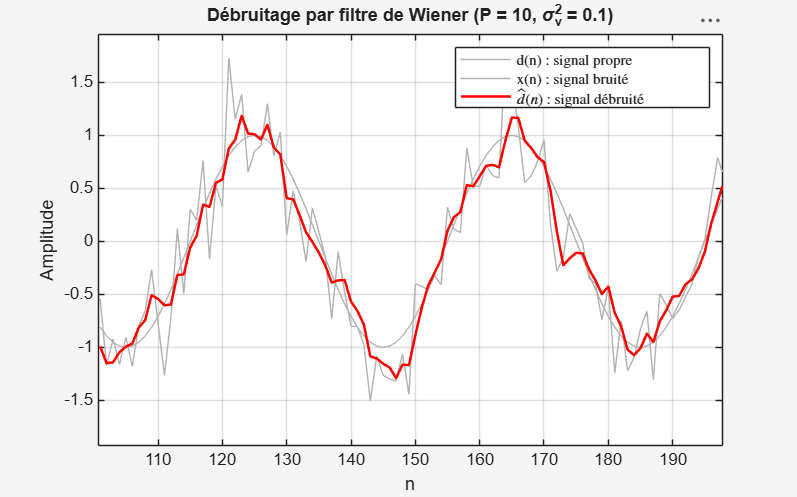
\includegraphics[width=0.9\linewidth]{fig21}
  \caption{Signal propre $d(n)$, signal bruité $x(n)$ et signal débruité $\hat d(n)$ ($P=10$, $\sigma_v^2=0.1$).}
\end{figure}

\begin{interpretation}
\begin{itemize}
  \item RSB avant débruitage : $10\log_{10}(0.5/0.1)\approx 7$~dB ; $x(n)$ fluctue fortement autour de la sinusoïde.
  \item $\hat d(n)$ est beaucoup plus lisse et suit $d(n)$ en phase et en amplitude. Le petit résidu restant est le bruit situé dans la bande passante du filtre, encore large pour $P=10$.
  \item Les $P-1$ premiers échantillons de $\hat d(n)$ sont un régime transitoire : la fenêtre affichée ($n=101$ à $200$) est choisie après cette zone.
\end{itemize}
\end{interpretation}

\subsection{Question (b) : valeur de \texorpdfstring{$\mathrm{EQM}_{\min}$}{EQMmin}}

\begin{enonce}
\textbf{Énoncé :} Déterminer la valeur de $\mathrm{EQM}_{\min}$ en utilisant son expression déduite dans le cours.
\end{enonce}

\textbf{Démarche.} On applique $\mathrm{EQM}_{\min}=r_d(0)-\mathbf{w}_{opt}^T\mathbf{r}_{dx}$, où $r_d(0)$ est la puissance de $d(n)$ (théoriquement $A^2/2=0.5$), soit le premier élément du vecteur \texttt{rd}.

\textbf{Code.} (à la suite du code de la question (a))
\begin{lstlisting}
% EQM_min selon la formule du cours ; rd(1) = r_d(0)
EQM_min = rd(1) - wopt' * rd;
fprintf('Valeur de l''EQM_min theorique (pour P = %d, sigma_v^2 = %.2f) : %.4f\n', P, sigv2, EQM_min);
\end{lstlisting}

\begin{figure}[H]
    \centering
    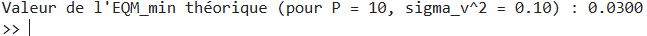
\includegraphics[width=0.85\linewidth]{fig22}
    \caption{Valeur de $\mathrm{EQM}_{\min}$ affichée dans la console ($P=10$, $\sigma_v^2=0.1$).}
\end{figure}

\begin{resultat}
$\mathrm{EQM}_{\min}=0.0300$ pour $P=10$ et $\sigma_v^2=0.1$.
\end{resultat}

\begin{interpretation}
\begin{itemize}
  \item C'est l'erreur minimale atteignable par un filtre RIF d'ordre $10$. Sans filtrage ($\hat d=x$), l'erreur vaut $\sigma_v^2=0.1$ : le filtre la divise par $3.3$, soit un gain de $10\log_{10}(0.1/0.03)\approx 5.2$~dB, cohérent avec le gain mesuré en (f) ($5.4$~dB pour $P=10$).
  \item Avec les corrélations exactes ($r_d(k)=\tfrac12\cos(kw_0)$), on obtient $\mathrm{EQM}_{\min}=0.0279$ : l'écart vient de l'estimation des corrélations sur $N=10^4$ échantillons (voir (d)).
\end{itemize}
\end{interpretation}

\subsection{Question (c) : convergence de \texorpdfstring{$eqm(k)$}{eqm(k)} pour P = 3, 5 et 10}

\begin{enonce}
\textbf{Énoncé :} Afficher l'EQM calculée en ligne $eqm(k)=\frac{1}{k}\sum_{i=1}^{k}(d(i)-\hat d(i))^2$, la stocker dans le vecteur \texttt{eqm} et montrer par simulation qu'elle converge vers $\mathrm{EQM}_{\min}$ pour $P=3$, $5$ et $10$. Afficher les courbes et les droites horizontales d'ordonnée $\mathrm{EQM}_{\min}$. Interpréter.
\end{enonce}

\textbf{Démarche.} Pour chaque $P$ : calcul de $\mathbf{w}_{opt}$, $\hat d(n)$ et $\mathrm{EQM}_{\min}$ ; calcul récursif de $eqm(k)=S_k/k$ avec $S_k=S_{k-1}+(d(k)-\hat d(k))^2$ ; tracé de $eqm(k)$ et de la droite $\mathrm{EQM}_{\min}$ (axe $k$ logarithmique).

\textbf{Code.} (script séparé : $d(n)$ et $x(n)$ sont générés comme en (a), avec un nouveau tirage du bruit)
\begin{lstlisting}
Plist  = [3 5 10];
EQM    = zeros(N, length(Plist));
EQMmin = zeros(1, length(Plist));

for m = 1:length(Plist)
    Pm  = Plist(m);
    rxm = xcorr(x, Pm-1, 'biased'); rxm = rxm(Pm:end);
    rdm = xcorr(d, Pm-1, 'biased'); rdm = rdm(Pm:end);
    wm  = toeplitz(rxm) \ rdm;
    dhm = filter(wm, 1, x);

    S = 0;
    for k = 1:N
        S        = S + (d(k) - dhm(k))^2;
        EQM(k,m) = S / k;
    end
    EQMmin(m) = rdm(1) - wm' * rdm;
    fprintf('P = %2d : EQM_min = %.4f | eqm(N) = %.4f\n', Pm, EQMmin(m), EQM(N,m));
end

% Une figure par P
for m = 1:length(Plist)
    figure;
    plot(1:N, EQM(:,m), 'b', 'LineWidth', 1.3); hold on;
    plot([1 N], [EQMmin(m) EQMmin(m)], 'r--', 'LineWidth', 1.3);
    set(gca, 'XScale', 'log'); grid on;
    ylim([0 3*EQMmin(m)]);
    xlabel('k'); ylabel('eqm(k)');
    title(sprintf('Convergence de eqm(k) vers EQM_{min} (P = %d)', Plist(m)));
    legend('eqm(k)', 'EQM_{min}', 'Location', 'best');
end

% Les trois courbes ensemble
col = lines(3);
figure; hold on;
for m = 1:length(Plist)
    h(m) = plot(1:N, EQM(:,m), 'Color', col(m,:), 'LineWidth', 1.3);
    plot([1 N], [EQMmin(m) EQMmin(m)], '--', 'Color', col(m,:), 'LineWidth', 1);
end
set(gca, 'XScale', 'log'); grid on;
ylim([0 3*max(EQMmin)]);
xlabel('k'); ylabel('eqm(k)');
legend(h, 'P = 3', 'P = 5', 'P = 10', 'Location', 'best');
\end{lstlisting}

\begin{figure}[H]
  \centering
  \begin{subfigure}{0.49\linewidth}
    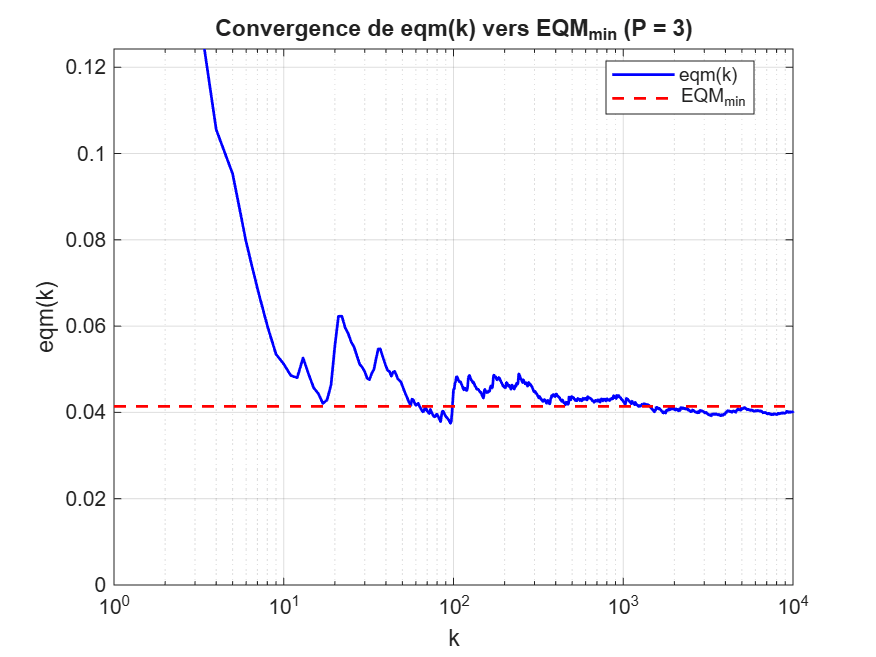
\includegraphics[width=\linewidth]{fig23}
    \caption{$P=3$}
  \end{subfigure}\hfill
  \begin{subfigure}{0.49\linewidth}
    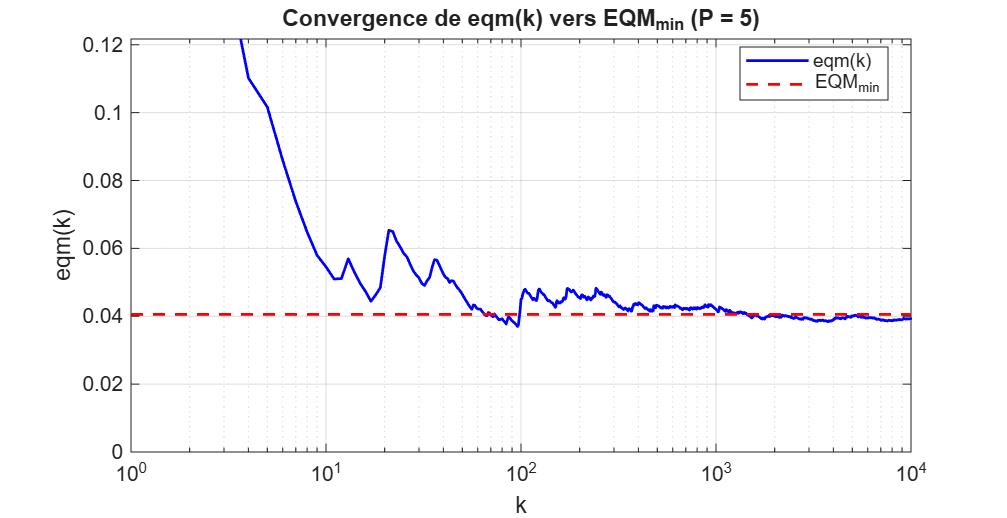
\includegraphics[width=\linewidth]{fig24}
    \caption{$P=5$}
  \end{subfigure}

  \medskip
  \begin{subfigure}{0.49\linewidth}
    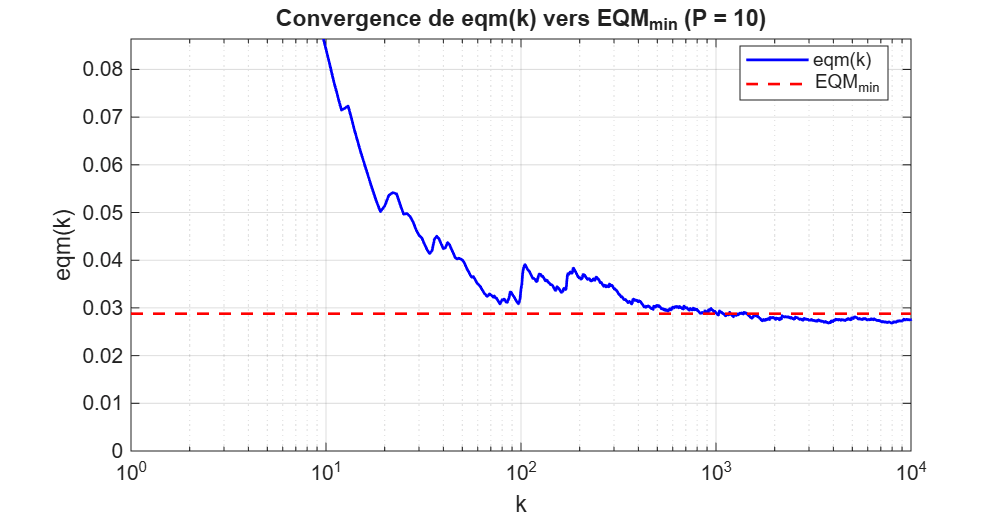
\includegraphics[width=\linewidth]{fig25}
    \caption{$P=10$}
  \end{subfigure}\hfill
  \begin{subfigure}{0.49\linewidth}
    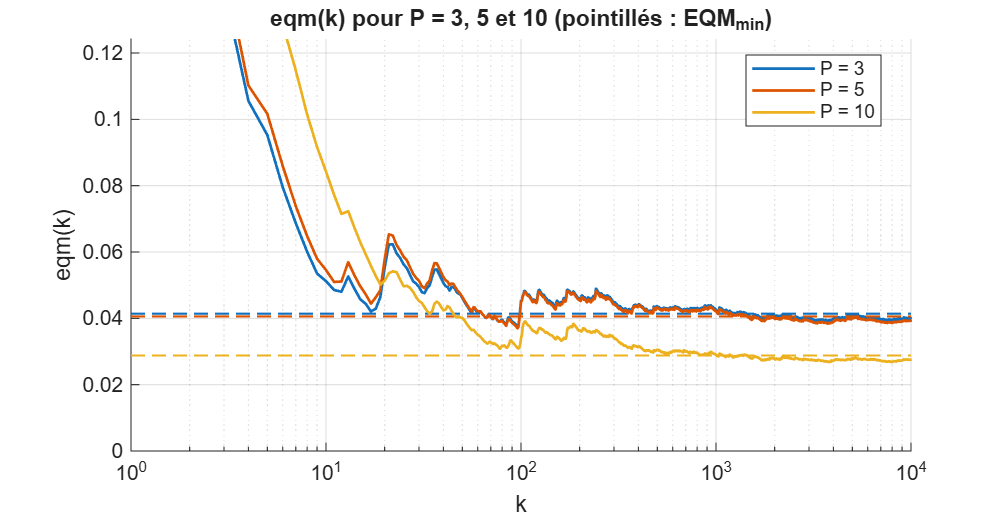
\includegraphics[width=\linewidth]{fig26}
    \caption{Comparaison des trois ordres}
  \end{subfigure}
  \caption{$eqm(k)$ (trait plein) et $\mathrm{EQM}_{\min}$ (pointillés) pour $\sigma_v^2=0.1$.}
\end{figure}

\begin{resultat}
$\mathrm{EQM}_{\min}\approx 0.041$ ($P=3$), $0.040$ ($P=5$) et $0.029$ ($P=10$). Pour chaque ordre, $eqm(k)$ converge vers $\mathrm{EQM}_{\min}$ à environ $10^{-3}$ près à partir de $k\approx 10^3$.\\
{\small (Nouvelle exécution du script, donc nouvelle réalisation du bruit : $0.029$ au lieu de $0.030$ en (b) pour $P=10$.)}
\end{resultat}

\begin{interpretation}
\begin{itemize}
  \item \textbf{Convergence.} La formule du cours donne bien l'erreur réellement obtenue : $eqm(k)$ est une moyenne empirique qui tend vers l'espérance $E[(d-\hat d)^2]=\mathrm{EQM}_{\min}$ (ergodicité).
  \item \textbf{Début des courbes.} L'erreur est élevée au départ à cause du régime transitoire du filtre (les $P-1$ premiers échantillons) et de la moyenne sur peu de points ; le poids de ces valeurs décroît en $1/k$.
  \item \textbf{Écart résiduel} (de l'ordre de $10^{-3}$) : erreur d'estimation des corrélations sur $N=10^4$ échantillons, étudiée en (d).
  \item \textbf{Influence de $P$.} $P=3$ et $P=5$ donnent presque la même erreur ; $P=10$ la réduit nettement : un filtre plus long a une bande passante plus étroite autour de $w_0$ et laisse passer moins de bruit.
\end{itemize}
\end{interpretation}

\subsection{Question (d) : influence de la puissance du bruit}

\begin{enonce}
\textbf{Énoncé :} Tracer la même courbe d'EQM pour $P=10$ et $\sigma_v^2\in\{0.01,\ 0.05,\ 0.1,\ 0.5,\ 1\}$. Interpréter.
\end{enonce}

\textbf{Démarche.} Pour chaque $\sigma_v^2$ : nouveau bruit, calcul de $\mathbf{w}_{opt}$, $\hat d(n)$, $\mathrm{EQM}_{\min}$ et $eqm(k)$ comme en (c). Une figure par valeur, puis une comparaison en échelle log--log. Le script est relancé avec $N=10^5$ pour vérifier l'écart observé à faible bruit.

\textbf{Code.}
\begin{lstlisting}
clear; clc; close all;

% Parametres
N       = 1e4;            % 1e5 pour la verification
n       = (1:N)';
w0      = 0.05*pi;
phi     = pi/4;
P       = 10;
sigList = [0.01 0.05 0.1 0.5 1];
nS      = length(sigList);

d = sin(n*w0 + phi);

EQM    = zeros(N, nS);
EQMmin = zeros(1, nS);

for s = 1:nS
    % Signal bruite pour cette valeur de sigv2
    x = d + sqrt(sigList(s))*randn(N,1);

    % Filtre de Wiener
    rx = xcorr(x, P-1, 'biased'); rx = rx(P:end);
    rd = xcorr(d, P-1, 'biased'); rd = rd(P:end);
    wopt = toeplitz(rx) \ rd;
    dhat = filter(wopt, 1, x);

    % eqm(k) calculee en ligne
    S = 0;
    for k = 1:N
        S        = S + (d(k) - dhat(k))^2;
        EQM(k,s) = S / k;
    end
    EQMmin(s) = rd(1) - wopt' * rd;
    fprintf('sigv2 = %.2f : EQM_min = %.4f | eqm(N) = %.4f\n', ...
            sigList(s), EQMmin(s), EQM(N,s));
end

% Une figure par sigv2
for s = 1:nS
    figure;
    plot(1:N, EQM(:,s), 'b', 'LineWidth', 1.3); hold on;
    plot([1 N], [EQMmin(s) EQMmin(s)], 'r--', 'LineWidth', 1.3);
    set(gca, 'XScale', 'log'); grid on;
    ylim([0 3*EQMmin(s)]);
    xlabel('k'); ylabel('eqm(k)');
    legend('eqm(k)', 'EQM_{min}', 'Location', 'best');
end

% Comparaison (axes log)
col = lines(nS);
figure; hold on;
for s = 1:nS
    h(s) = plot(1:N, EQM(:,s), 'Color', col(s,:), 'LineWidth', 1.3);
    plot([1 N], [EQMmin(s) EQMmin(s)], '--', 'Color', col(s,:));
end
set(gca, 'XScale', 'log', 'YScale', 'log'); grid on;
ylim([0.5*min(EQMmin) 3*max(EQMmin)]);
xlabel('k'); ylabel('eqm(k)');
legend(h, arrayfun(@(v) sprintf('\\sigma_v^2 = %.2f', v), sigList, ...
       'UniformOutput', false), 'Location', 'best');
\end{lstlisting}

\begin{figure}[H]
  \centering
  \begin{subfigure}{0.49\linewidth}
    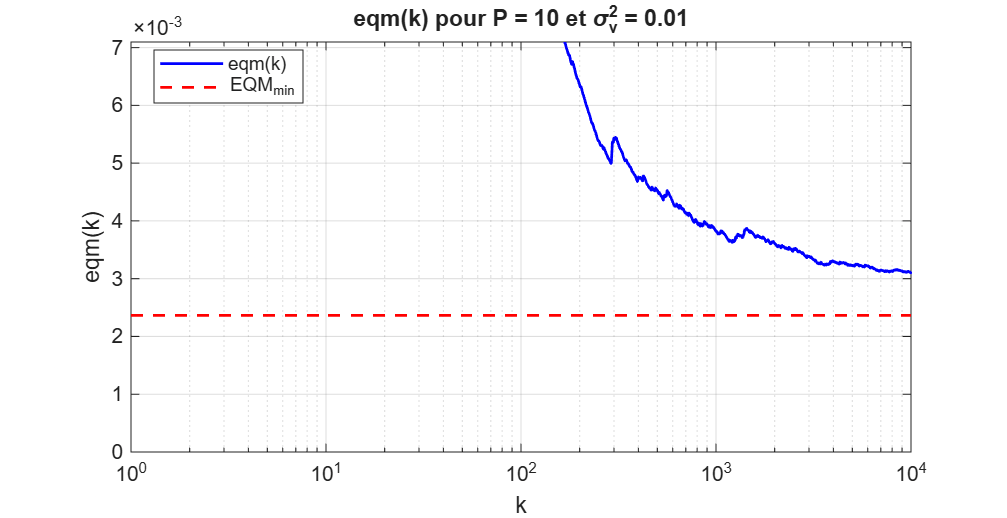
\includegraphics[width=\linewidth]{fig27}
    \caption{$\sigma_v^2=0.01$}
  \end{subfigure}\hfill
  \begin{subfigure}{0.49\linewidth}
    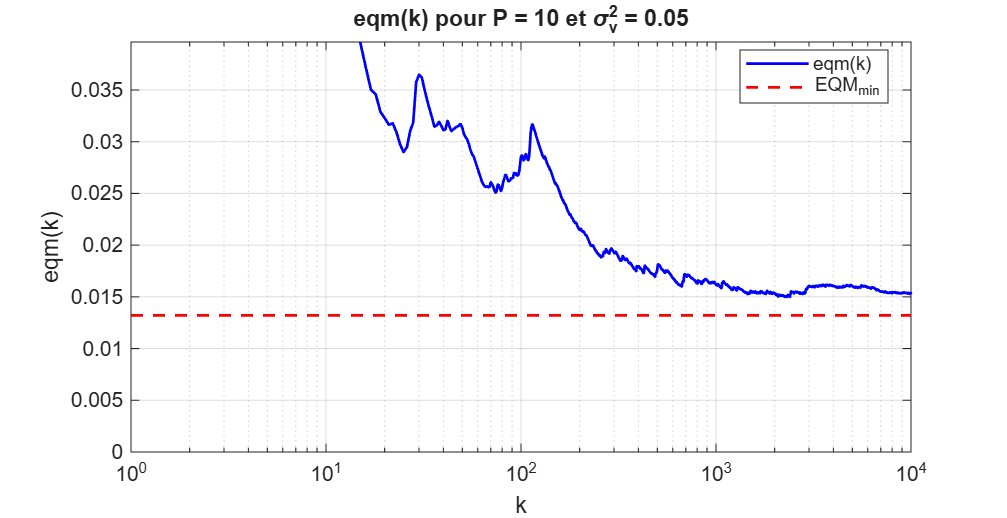
\includegraphics[width=\linewidth]{fig28}
    \caption{$\sigma_v^2=0.05$}
  \end{subfigure}

  \medskip
  \begin{subfigure}{0.49\linewidth}
    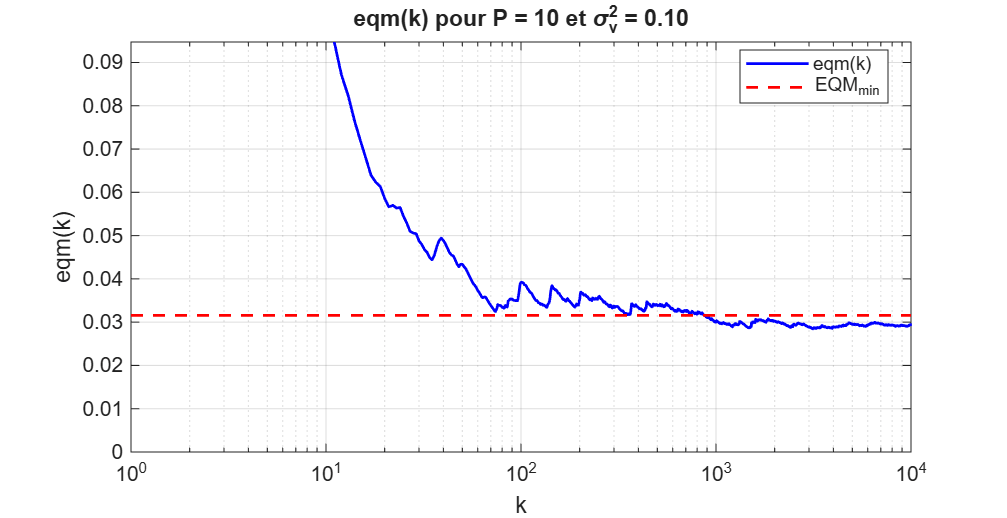
\includegraphics[width=\linewidth]{fig29}
    \caption{$\sigma_v^2=0.1$}
  \end{subfigure}\hfill
  \begin{subfigure}{0.49\linewidth}
    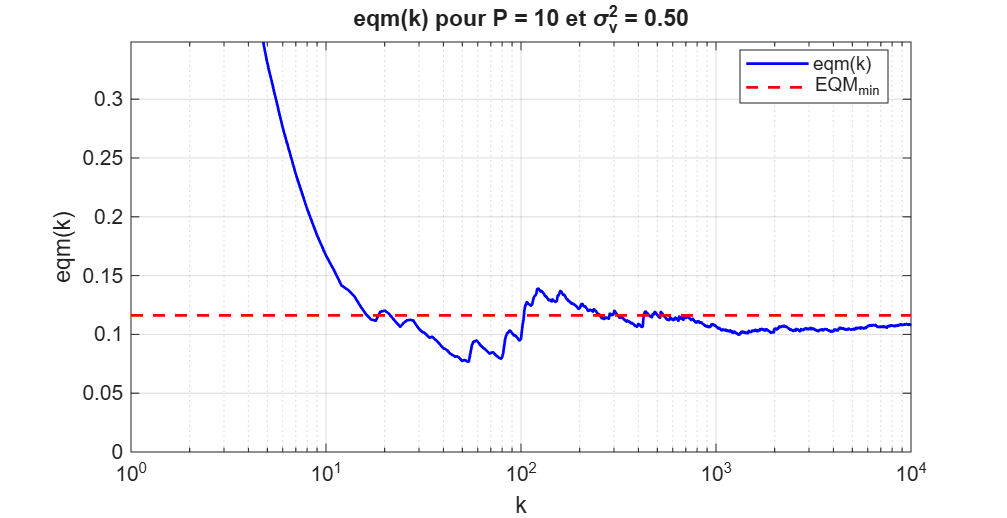
\includegraphics[width=\linewidth]{fig30}
    \caption{$\sigma_v^2=0.5$}
  \end{subfigure}

  \medskip
  \begin{subfigure}{0.49\linewidth}
    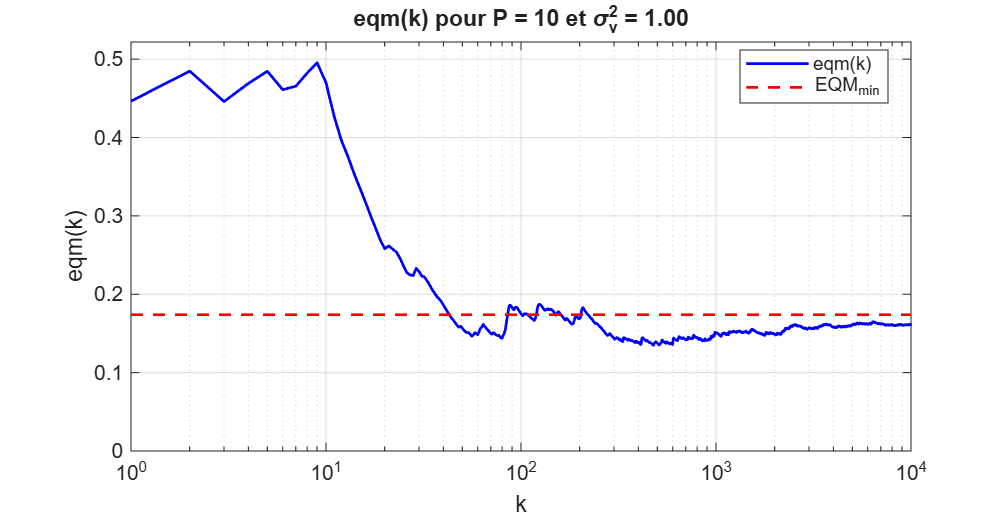
\includegraphics[width=\linewidth]{fig31}
    \caption{$\sigma_v^2=1$}
  \end{subfigure}
  \caption{$eqm(k)$ et $\mathrm{EQM}_{\min}$ pour $P=10$ et les différentes valeurs de $\sigma_v^2$ ($N=10^4$).}
\end{figure}

\begin{figure}[H]
  \centering
  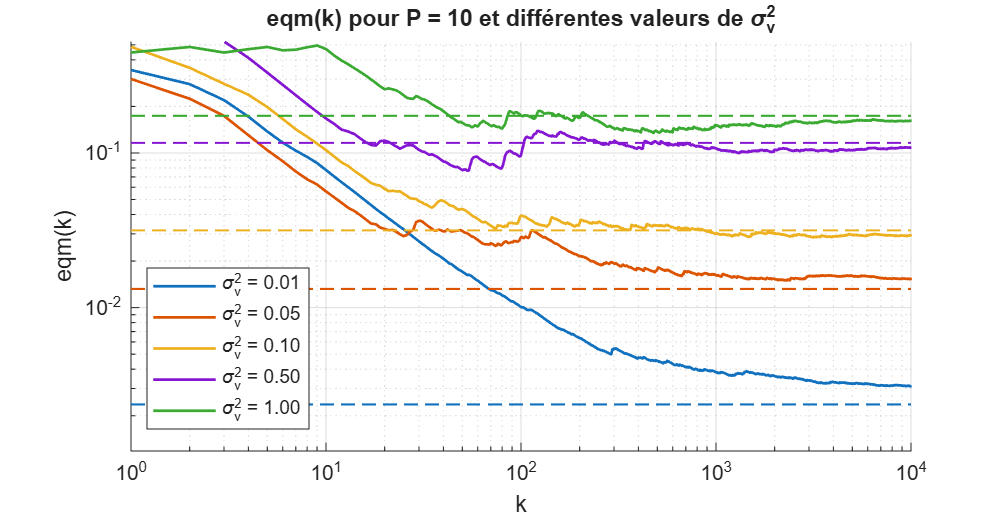
\includegraphics[width=0.8\linewidth]{fig32}
  \caption{Comparaison de $eqm(k)$ pour $P=10$ (pointillés : $\mathrm{EQM}_{\min}$ correspondants), $N=10^4$.}
  \label{fig:comp1e4}
\end{figure}

\begin{figure}[H]
  \centering
  \begin{subfigure}{0.49\linewidth}
    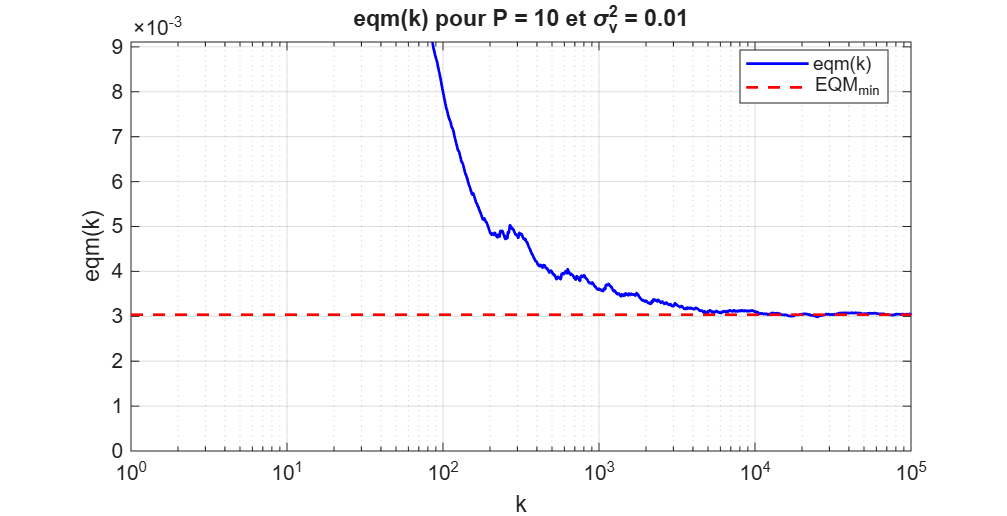
\includegraphics[width=\linewidth]{fig33}
    \caption{$\sigma_v^2=0.01$}
    \label{fig:verif1}
  \end{subfigure}\hfill
  \begin{subfigure}{0.49\linewidth}
    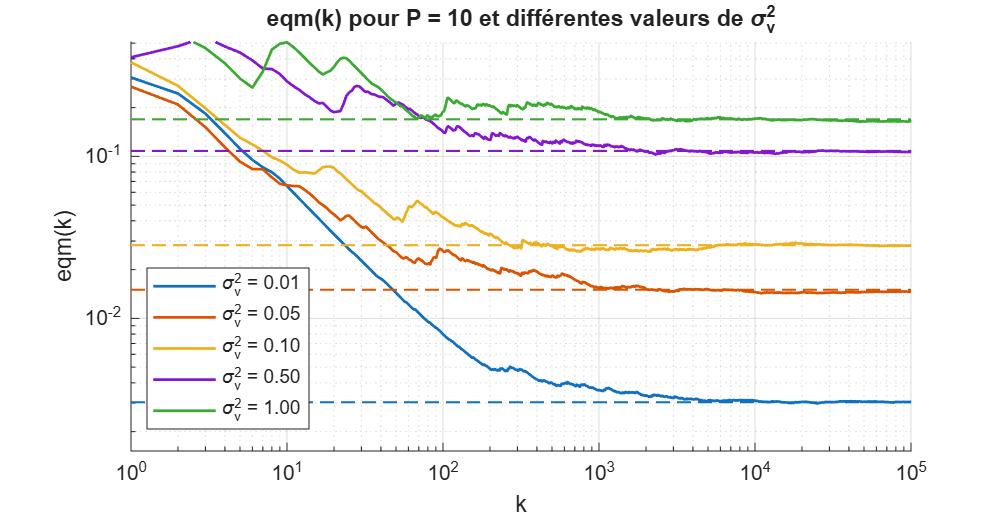
\includegraphics[width=\linewidth]{fig34}
    \caption{Toutes les valeurs de $\sigma_v^2$}
    \label{fig:verif2}
  \end{subfigure}
  \caption{Vérification avec $N=10^5$ échantillons ($P=10$).}
\end{figure}

\begin{table}[H]
  \centering
  \begin{tabular}{cccc}
    \toprule
    $\sigma_v^2$ & $\mathrm{EQM}_{\min}$ (formule, $N=10^4$) & $eqm(N)$ mesurée ($N=10^4$) & $\mathrm{EQM}_{\min}$ théorique \\
    \midrule
    $0.01$ & $0.0024$ & $0.0031$ & $0.0030$ \\
    $0.05$ & $0.013$  & $0.015$  & $0.015$ \\
    $0.1$  & $0.032$  & $0.029$  & $0.028$ \\
    $0.5$  & $0.116$  & $0.108$  & $0.107$ \\
    $1$    & $0.173$  & $0.161$  & $0.168$ \\
    \bottomrule
  \end{tabular}
  \caption{Erreurs obtenues pour $P=10$. La colonne théorique utilise les corrélations exactes $r_d(k)=\tfrac12\cos(kw_0)$ et $r_x(k)=r_d(k)+\sigma_v^2\delta(k)$.}
\end{table}

\begin{interpretation}
\begin{itemize}
  \item \textbf{Effet du bruit.} $\mathrm{EQM}_{\min}$ augmente avec $\sigma_v^2$ : avec $P=10$ coefficients, le résidu de bruit croît avec la puissance du bruit. Elle reste toujours inférieure à $\sigma_v^2$ (erreur sans filtrage) : le filtre réduit le bruit dans tous les cas.
  \item \textbf{Écart entre $eqm(N)$ et $\mathrm{EQM}_{\min}$.} Les courbes se stabilisent, mais pas exactement sur la droite (écart de signe variable). C'est une \emph{erreur d'estimation} de $\mathrm{EQM}_{\min}$ : la formule suppose $r_{dx}(k)=r_d(k)$, alors que l'intercorrélation estimée entre $d$ et $v$ n'est pas nulle sur $10^4$ échantillons. L'écart relatif est faible à fort bruit ($\approx 7\,\%$ pour $\sigma_v^2=0.5$ et $1$) mais important pour $\sigma_v^2=0.01$ ($0.0024$ contre $0.0031$, soit $\approx 25\,\%$).
  \item \textbf{Vérification ($N=10^5$).} Pour $\sigma_v^2=0.01$, $\mathrm{EQM}_{\min}$ passe à $0.0030$, égale à la valeur théorique, et $eqm(k)$ converge vers elle ; toutes les courbes rejoignent alors leur droite (figure~\ref{fig:verif2}). L'erreur d'estimation diminue donc quand $N$ augmente.
  \item \textbf{Vitesse de convergence.} Elle est plus lente à faible bruit : l'erreur initiale (transitoire), divisée par $k$, doit devenir négligeable devant une $\mathrm{EQM}_{\min}$ très petite ($k\approx 10^3$--$10^4$ pour $\sigma_v^2=0.01$, contre $10^2$--$10^3$ pour les autres).
\end{itemize}
\end{interpretation}

\subsection{Question (e) : \texorpdfstring{$\mathrm{EQM}_{\min}$}{EQMmin} en fonction de l'ordre P}

\begin{enonce}
\textbf{Énoncé :} On fixe $\sigma_v^2=0.1$. Tracer $\mathrm{EQM}_{\min}$ en fonction de $P$, pour $P$ variant de $5$ à $50$ avec un pas de $5$. Interpréter.
\end{enonce}

\textbf{Démarche.} Une seule réalisation de $x(n)$ est utilisée pour tous les ordres, afin que seul $P$ change. Pour chaque $P$, on calcule $\mathrm{EQM}_{\min}$ (formule) et, pour contrôle, l'erreur mesurée $eqm(N)$.

\textbf{Code.}
\begin{lstlisting}
clear; clc; close all;

% Parametres
N     = 1e4;
n     = (1:N)';
w0    = 0.05*pi;
phi   = pi/4;
sigv2 = 0.1;
Plist = 5:5:50;
nP    = length(Plist);

% Signal propre et signal bruite (meme realisation pour tous les P)
d = sin(n*w0 + phi);
x = d + sqrt(sigv2)*randn(N,1);

EQMmin = zeros(1, nP);
eqmN   = zeros(1, nP);

for m = 1:nP
    P = Plist(m);

    % Filtre de Wiener d'ordre P
    rx = xcorr(x, P-1, 'biased'); rx = rx(P:end);
    rd = xcorr(d, P-1, 'biased'); rd = rd(P:end);
    wopt = toeplitz(rx) \ rd;
    dhat = filter(wopt, 1, x);

    % EQM_min (formule)
    EQMmin(m) = rd(1) - wopt' * rd;

    % eqm(N) mesuree
    S = 0;
    for k = 1:N
        S = S + (d(k) - dhat(k))^2;
    end
    eqmN(m) = S / N;

    fprintf('P = %2d : EQM_min = %.4f | eqm(N) = %.4f\n', ...
            P, EQMmin(m), eqmN(m));
end

% EQM_min et eqm(N) en fonction de P
figure;
plot(Plist, EQMmin, 'b-o', 'LineWidth', 1.3, 'MarkerFaceColor', 'b'); hold on;
plot(Plist, eqmN, 'r--s', 'LineWidth', 1.3);
grid on; xticks(Plist);
xlabel('Ordre P'); ylabel('EQM');
legend('EQM_{min} (formule)', 'eqm(N) (mesuree)', 'Location', 'best');
\end{lstlisting}

\begin{figure}[H]
  \centering
  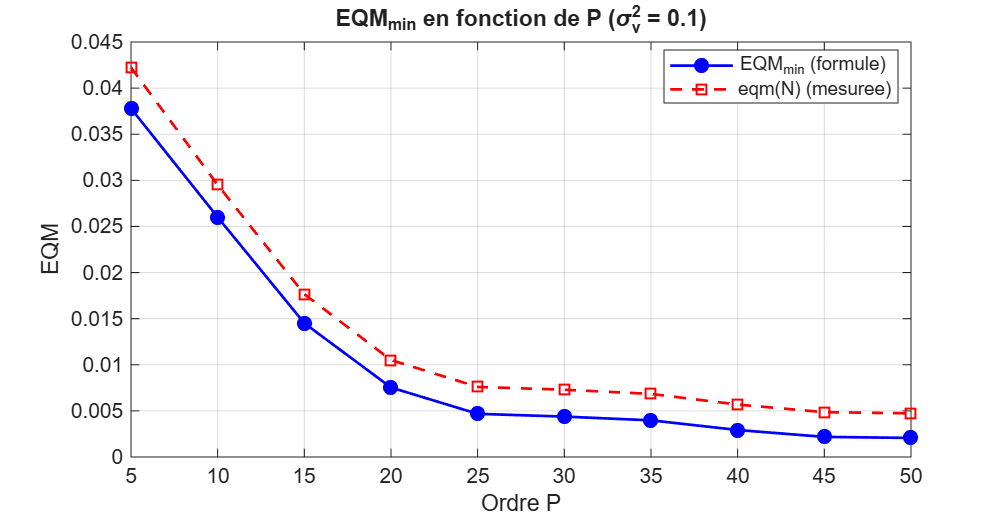
\includegraphics[width=0.8\linewidth]{fig35}
  \caption{$\mathrm{EQM}_{\min}$ (formule) et $eqm(N)$ (mesurée) en fonction de $P$ ($\sigma_v^2=0.1$).}
\end{figure}

\begin{interpretation}
\begin{itemize}
  \item \textbf{Tendance.} $\mathrm{EQM}_{\min}$ diminue avec $P$ : forte baisse de $P=5$ à $P=20$ ($0.0378\to 0.0075$, division par 5), puis palier ($0.0047$ à $P=25$, $0.0021$ à $P=50$).
  \item \textbf{Explication fréquentielle.} Le bruit blanc occupe toutes les fréquences, le signal est concentré en $w_0$. Un filtre plus long a une bande passante plus étroite autour de $w_0$ : il élimine plus de bruit sans toucher à la sinusoïde. Une fois la bande assez étroite, l'allonger n'apporte presque plus rien.
  \item \textbf{Mesure.} $eqm(N)$ suit la même tendance mais reste toujours au-dessus de $\mathrm{EQM}_{\min}$ (écart de $0.0045$ à $P=5$, $0.0026$ à $P=50$) : c'est l'erreur d'estimation vue en (d), de même signe ici car la réalisation du bruit est la même pour tous les $P$.
  \item \textbf{Conclusion.} Au-delà de $P\approx 25$, le gain en erreur est faible alors que le coût augmente (matrice $\mathbf{R}_x$ plus grande, transitoire plus long).
\end{itemize}
\end{interpretation}

\subsection{Question (f) : gain en RSB et choix de l'ordre P}

\begin{enonce}
\textbf{Énoncé :} Le gain en RSB après débruitage est défini par $\mathrm{gain}|_{\mathrm{dB}}=\mathrm{RSB}|_{\mathrm{ap}}-\mathrm{RSB}|_{\mathrm{av}}$. Afficher la courbe de $\mathrm{gain}|_{\mathrm{dB}}$ en faisant varier $P$ comme en (e). Interpréter. Quel est le meilleur choix de l'ordre $P$ ?
\end{enonce}

\textbf{Démarche.} Avant débruitage, l'erreur est $v(n)$ ; après, c'est $e(n)=d(n)-\hat d(n)$ :
\[
\mathrm{RSB}_{\mathrm{av}}=10\log_{10}\frac{P_d}{P_v},\qquad
\mathrm{RSB}_{\mathrm{ap}}=10\log_{10}\frac{P_d}{P_e},\qquad
\mathrm{gain}|_{\mathrm{dB}}=10\log_{10}\frac{P_v}{P_e}.
\]
Les puissances sont calculées par moyennes temporelles. On trace aussi le gain déduit de la formule, $10\log_{10}(P_v/\mathrm{EQM}_{\min})$.

\textbf{Code.}
\begin{lstlisting}
clear; clc; close all;

% Parametres
N     = 1e4;
n     = (1:N)';
w0    = 0.05*pi;
phi   = pi/4;
sigv2 = 0.1;
Plist = 5:5:50;
nP    = length(Plist);

% Signal propre et signal bruite (meme realisation pour tous les P)
d = sin(n*w0 + phi);
v = sqrt(sigv2)*randn(N,1);
x = d + v;

% Puissances du signal et du bruit
Sd = 0; Sv = 0;
for k = 1:N
    Sd = Sd + d(k)^2;
    Sv = Sv + v(k)^2;
end
Pd = Sd / N;
Pv = Sv / N;

% RSB avant debruitage
RSBav = 10*log10(Pd / Pv);

RSBap  = zeros(1, nP);
gain   = zeros(1, nP);
gainTh = zeros(1, nP);

for m = 1:nP
    P = Plist(m);

    % Filtre de Wiener d'ordre P
    rx = xcorr(x, P-1, 'biased'); rx = rx(P:end);
    rd = xcorr(d, P-1, 'biased'); rd = rd(P:end);
    wopt = toeplitz(rx) \ rd;
    dhat = filter(wopt, 1, x);
    EQMmin = rd(1) - wopt' * rd;

    % Puissance de l'erreur residuelle
    Se = 0;
    for k = 1:N
        Se = Se + (d(k) - dhat(k))^2;
    end
    Pe = Se / N;

    % RSB apres debruitage et gain
    RSBap(m)  = 10*log10(Pd / Pe);
    gain(m)   = RSBap(m) - RSBav;
    gainTh(m) = 10*log10(Pv / EQMmin);
end

% Gain en fonction de P
figure;
plot(Plist, gain, 'b-o', 'LineWidth', 1.3, 'MarkerFaceColor', 'b'); hold on;
plot(Plist, gainTh, 'r--s', 'LineWidth', 1.3);
grid on; xticks(Plist);
xlabel('Ordre P'); ylabel('gain (dB)');
legend('gain mesure', 'gain deduit de EQM_{min}', 'Location', 'best');
\end{lstlisting}

\begin{figure}[H]
  \centering
  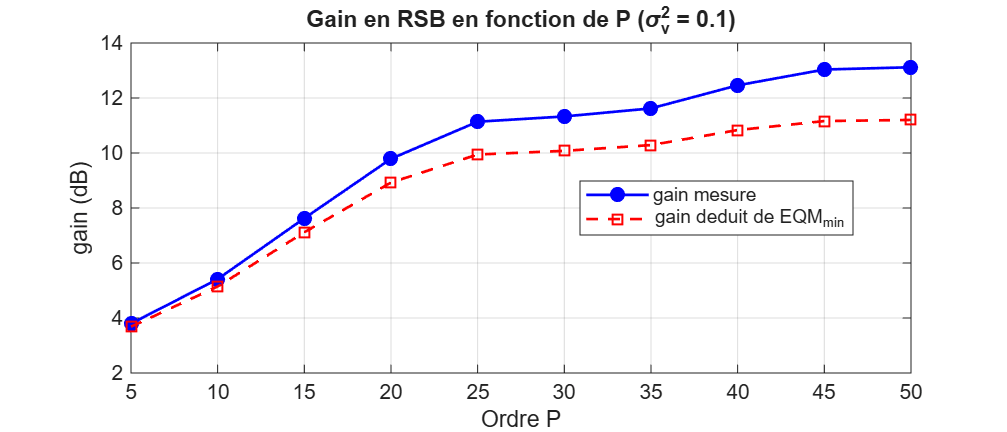
\includegraphics[width=0.8\linewidth]{fig36}
  \caption{Gain en RSB (mesuré et déduit de $\mathrm{EQM}_{\min}$) en fonction de $P$ ($\sigma_v^2=0.1$).}
\end{figure}

\begin{interpretation}
\begin{itemize}
  \item \textbf{RSB initial.} $P_d=0.5$, $P_v=0.098$, donc $\mathrm{RSB}_{\mathrm{av}}=7.08$~dB.
  \item \textbf{Évolution du gain.} $3.80$~dB ($P=5$), $5.4$~dB ($P=10$), $9.79$~dB ($P=20$), $11.14$~dB ($P=25$), puis seulement $13.12$~dB à $P=50$. Comme $\mathrm{gain}|_{\mathrm{dB}}=10\log_{10}(P_v/P_e)$, la courbe est le miroir de celle de (e) : forte hausse, puis palier.
  \item \textbf{Gain déduit de $\mathrm{EQM}_{\min}$.} Même tendance, mais en dessous du gain mesuré (écart de $0.1$~dB à $P=5$ à $1.9$~dB à $P=50$). L'écart est de sens inverse de celui de (e), car ce script utilise une autre réalisation du bruit : c'est bien une erreur d'estimation aléatoire, plus visible en dB quand l'erreur est petite (grands $P$).
\end{itemize}
\end{interpretation}

\begin{resultat}[Meilleur choix de l'ordre]
$P\approx 25$ : environ $11$~dB de gain, soit l'essentiel de l'amélioration possible. Au-delà, doubler l'ordre n'apporte que $\approx 2$~dB (du même ordre que l'incertitude d'estimation) pour un coût de calcul et un transitoire plus grands.
\end{resultat}
